%!TEX root = ../Bachelorseminar-RoboticSwarms.tex


%-------------------
%NOTES
%
%- scalability, global communication, 
%- lots of overlap

In the previous sections, we reviewed the main problems found in the field of robotic swarms. 
However, these problems often overlap.
This is because the problems found in this field often consist of multiple different problems. 
We focused on each problem, highlighting the communication methods of every solution and properties of these communication methods. 
We summarize these properties in a Venn-diagram \ref{fig:AlgorithmsOverview}, allowing for a compact overview of these solutions. 

	\begin{figure}[!ht]
		\caption{Venn Diagram; overview of algorithms}
		\label{venn_diagram}

		\centering

		\def\loclb{(180:2.0cm) circle (2.0cm)}
	  	\def\loclf{(0:2.0cm) circle (2.0cm)}
	  	\def\locrb{(90:2.0cm) circle (2.0cm)}
	  	\def\locrf{(270:2.0cm) circle (2.0cm)}

	    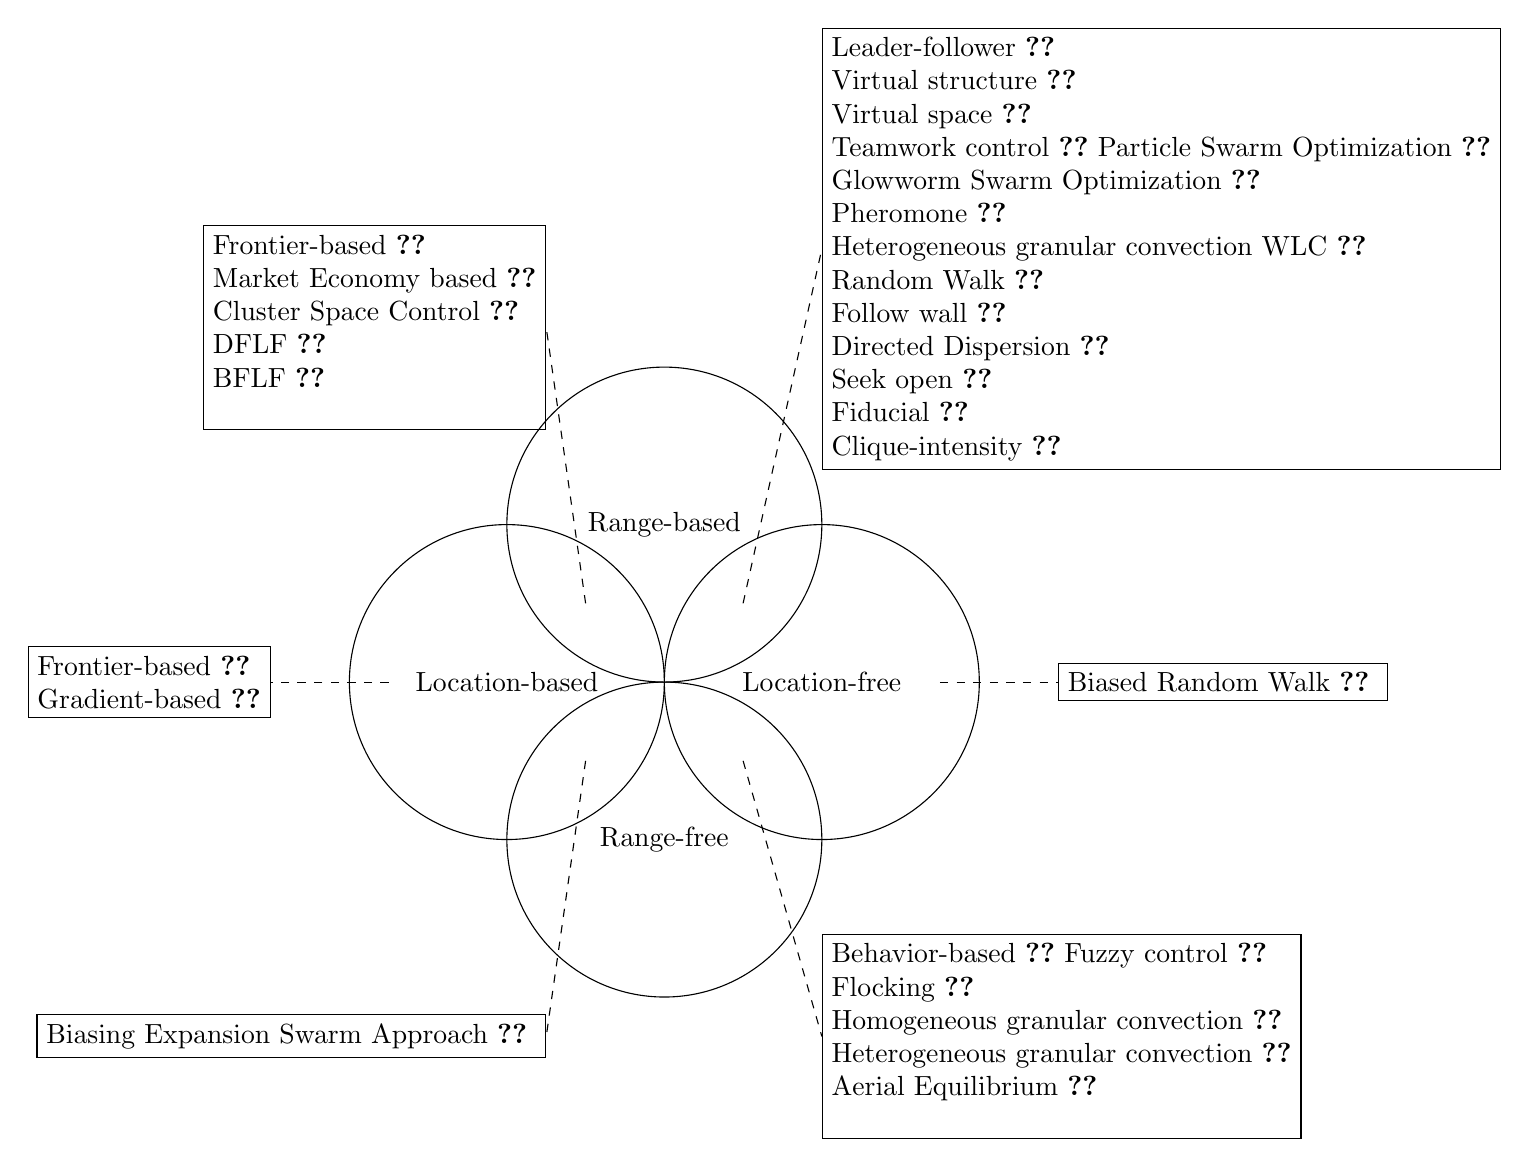
\begin{tikzpicture}
			% standard figures
			\draw \loclb node [text=black] {Location-based};
			\draw \loclf node [text=black] {Location-free};
			\draw \locrb node [text=black] {Range-based};
			\draw \locrf node [text=black] {Range-free};

			% Range-based location-free
			\draw[dashed,-] (1,1) -- (2,5.5) node[anchor=north west] {};
			\node[draw,align=left,anchor=west] at (2,5.5) {
				Leader-follower \ref{sec:Formation}\\
				Virtual structure \ref{sec:Formation}\\
				Virtual space \ref{sec:Formation}\\
				Teamwork control \ref{sec:Formation}
				Particle Swarm Optimization \ref{sec:Localization}\\
				Glowworm Swarm Optimization \ref{sec:Localization}\\
				Pheromone \ref{sec:CollectiveTransport}\\
				Heterogeneous granular convection WLC \ref{sec:CollectiveTransport}\\
				Random Walk \ref{sec:Dispersion}\\
				Follow wall \ref{sec:Dispersion}\\
				Directed Dispersion \ref{sec:Dispersion}\\
				Seek open \ref{sec:Dispersion}\\
				Fiducial \ref{sec:Dispersion}\\
				Clique-intensity \ref{sec:Dispersion}
			};

			% Range-free, location-free
			\draw[dashed,-] (1,-1) -- (2,-4.5) node[anchor=north west] {};
			\node[draw,align=left,anchor=west] at (2,-4.5) {
				Behavior-based \ref{sec:Formation}
				Fuzzy control \ref{sec:Formation}\\
				Flocking \ref{sec:CollectiveTransport}\\
				Homogeneous granular convection \ref{sec:CollectiveTransport}\\
				Heterogeneous granular convection \ref{sec:CollectiveTransport}\\
				Aerial Equilibrium \ref{sec:CollectiveTransport}\\
				%Virtual Pheromone \ref{sec:Path-planning}\\
				%Cardinality \ref{sec:Path-planning}
			};

			% location-free
			\draw[dashed,-] (3.5,0) -- (5,0) node[anchor=north west] {};
			\node[draw,align=left,anchor=west] at (5,0) {
				Biased Random Walk \ref{sec:Localization}
			};

			% location-based
			\draw[dashed,-] (-3.5,0) -- (-5,0) node[anchor=north west] {};
			\node[draw,align=left,anchor=east] at (-5,0) {
				Frontier-based \ref{sec:Exploration}\\
				Gradient-based \ref{sec:Localization}
			};

			% Range-free, location-based
			\draw[dashed,-] (-1,-1) -- (-1.5,-4.5) node[anchor=north west] {};
			\node[draw,align=left,anchor=east] at (-1.5,-4.5) {
				Biasing Expansion Swarm Approach \ref{sec:Localization}
			};

			% Range-based, location-based
			\draw[dashed,-] (-1,1) -- (-1.5,4.5) node[anchor=north west] {};
			\node[draw,align=left,anchor=east] at (-1.5,4.5) {
				Frontier-based \ref{sec:Exploration}\\
				Market Economy based \ref{sec:Exploration}\\
				Cluster Space Control \ref{sec:CollectiveTransport}\\
				DFLF \ref{sec:Dispersion}\\
				BFLF \ref{sec:Dispersion}\\
				%Artificial Bee Colony \ref{sec:Path-planning}\\
				%Multihop Communication \ref{sec:Path-planning}\\
				%Genetic Programming \ref{sec:Path-planning}
			};

			% Range-based
			%\draw[dashed,-] (0,3) -- (0,4.5) node[anchor=north west] {};
			%\node[draw,align=left,anchor=south] at (0,4.5) {

			%};

			% Range-free
			%\draw[dashed,-] (0,-3) -- (0,-4.5) node[anchor=north west] {};
			%\node[draw,align=left,anchor=north] at (0,-4.5) {
			
			%};
		\end{tikzpicture}
    \end{figure}


Throughout the suvery we have made the following observation about range usage and location usage. When using a location-free approach, the algorithm is overall really adaptable to dynamic environments. Some downsides is that this approach can require lots of central communication, which can make the scalability relatively low. When using a location-based approach, we observe very optimal solutions, however these solution only remain to be optimal if the algorithm is used in a static environment. Otherwise some basic algorithms such as collision-detection algorithms have to kick in, which can increase the overall runtime of the algorithm. Range-based algorithms allow for very dynamic environments and is one of the most important approaches due to its extreme usage of distributed intelligence. Range-free algorithms on the other side are not very scalable and do not make use of efficient cooperation.

- voornamelijk location-free
	- want maps moeten gemerged, bijgehouden worden gedeeld...

- location-based voornamelijk exploration algoritmes
	range-free location-free -> goed omdat gebruik bijv van wireless intensity signals erg onnauwkeurig is, non-optimal use of full robotic swarm
	range-based location-free -> want maps moeten gemerged, bijgehouden worden gedeeld... en dynamische omgeving kan in de gaten gehouden worden
	range-based -> belangrijkste gedeelte van een swarm, omdat daar de distributed intelligence ligt en dat daar het meeste onderzoek naar gedaan moet worden
	location-based -> kan ook handig zijn in statische locaties, als er rekening gehouden wordt met de scalability van de swarm  
	range-free -> matig scalable, maakt niet gebruik van efficiente samenwerking
- range-based �n range-free
	



Most algorithms are location-free.
This makes sense, as location-based solutions are not the most desirable, although they do provide high performance.
This is mainly because of three reasons. 
The first reason is cost. 
When an algorithm is location-based and range-based, the robots used in the swarm generally have to be equipped with advanced sensors. 
The robots are then more costly in terms of energy consumption and device price, which is not desirable.
The second reason is scalability. 
When an algorithm is location-based, most often centralized communication is needed. 
This introduces a lot of overhead, decreasing communication speed when robotic swarms increase in size. 
The third reason is that algorithms that are location-based can often not be used in dynamic locations, like underwater, space and underground environment.
This is especially true for algorithms where the operating environment has to be defined beforehand.\\

This survey, only highlighted a few problems that the robotic swarms technology has faced. 
Thus, more research on this topic needs to be undertaken on additional problems, such as mapping, foraging, target localization and robot localization, in order to create a fully comprehensive overview.

